\documentclass[11pt]{article}
\usepackage{graphicx,bm,amssymb,amsmath,amsthm}
% timo macros...
\newcommand{\bx}{\textbf{x}}
\newcommand{\by}{\textbf{y}}
\newcommand{\bs}{\textbf{s}}

% alex macros...
\newcommand{\bi}{\begin{itemize}}
\newcommand{\ei}{\end{itemize}}
\newcommand{\ben}{\begin{enumerate}}
\newcommand{\een}{\end{enumerate}}
\newcommand{\be}{\begin{equation}}
\newcommand{\ee}{\end{equation}}
\newcommand{\bea}{\begin{eqnarray}}
\newcommand{\eea}{\end{eqnarray}}
\newcommand{\bc}{\begin{center}}
\newcommand{\ec}{\end{center}}
\newcommand{\bfi}{\begin{figure}}
\newcommand{\efi}{\end{figure}}
\newcommand{\ca}[2]{\caption{#1 \label{#2}}}
\newcommand{\ig}[2]{\includegraphics[#1]{#2}}
\newcommand{\spl}[2]{\left\{\begin{array}{ll}#1\\#2\end{array}\right.}
\newcommand{\ie}{{\it i.e.\ }}
\newcommand{\eg}{{\it e.g.\ }}
\newcommand{\pd}[2]{\frac{\partial #1}{\partial #2}}
\newcommand{\pdc}[3]{\left. \frac{\partial #1}{\partial #2}\right|_{#3}}
\newcommand{\infint}{\int_{-\infty}^{\infty} \!\!}      % infinite integral
\newcommand{\tbox}[1]{{\mbox{\tiny #1}}}
\newcommand{\mbf}[1]{{\bm #1}}           % requires bm package
\newcommand{\pO}{{\partial\Omega}}
\newcommand{\uN}{u^{(N)}}
\newcommand{\emach}{\epsilon_\tbox{mach}}
%\newcommand{\crk}{C_{s}} %C_{R,k}         % const for exponential s(m) bnd
\newcommand{\bmp}[1]{\begin{minipage}{#1}}
\newcommand{\emp}{\end{minipage}}
\newcommand{\re}{\mbox{Re}\,}
\newcommand{\im}{\mbox{Im}\,}

\newtheorem{thm}{Theorem}
\newtheorem{cnj}{Conjecture}
\newtheorem{lem}{Lemma}[thm]
\newtheorem{cor}{Corollary}[thm]

\newtheorem{rmk}[thm]{Remark}
\newtheorem{pro}[thm]{Proposition}
%\newtheorem{cnj}[thm]{Conjecture}
%\newtheorem{lemma}[thm]{Lemma}

\newcommand{\bp}{{\bf Proof:\ }}   % {\begin{proof}}
\newcommand{\ep}{\hfill $\square$ \vspace{1ex} \\} % {\end{proof}}
% note elsart ones horrible: \pr and \endpr
\newcommand{\bmal}{{\bm \alpha}}             % bold alpha
\newcommand{\splt}[2]{$\left\{\begin{array}{l}\mbox{#1}\\\mbox{#2}\end{array}\ri
ght.$}
\newcommand{\lo}{{L^2(\Omega)}}
\newcommand{\lpo}{{L^2(\pO)}}
\newcommand{\cu}{\tilde{u}}            % symbol for continuation of u
\newcommand{\cOmega}{\tilde{\Omega}}   % symbol for domain to be continued into
\newcommand{\dmax}{D_\tbox{max}}       % max dist in splane_charge_curve

% spacers...
\newcommand{\tw}{\textwidth}
\newcommand{\vg}{\vspace{2ex}}

% brand names... the problem with putting a trailing space here is that then
% punctuation following the word cannot be correct. To use these with correct
% trailing space, use as \mpspack\ or \matlab\ or with ending period, \matlab.
\newcommand{\mpspack}{{\tt MPSpack}}            % name of this package
\newcommand{\matlab}{{M{\small ATLAB}}}            % name of MATLAB

% code formatting... (nearly ok, gets multiple-line padding wrong)
\newcommand{\co}[1]{\vspace{.5ex}
\\
\mbox{}\hspace{5ex}\begin{minipage}{\textwidth}{\tt #1}\end{minipage}%
\vspace{.5ex}%
\\}



\begin{document}
\title{\mpspack\ tutorial}
\author{Alex Barnett\footnote{Department of Mathematics, Dartmouth College,
Hanover, NH, 03755, USA}
\ and
Timo Betcke\footnote{Department of Mathematics,
University of Reading, Berkshire, RG6 6AX, UK}}
\date{\today}   % how pipe from getrevisionnumber + 1?

\maketitle
\begin{abstract}
This tutorial shows how a variety of two-dimensional Laplace and Helmholtz
boundary-value problems
may be numerically solved simply and accurately with the \mpspack\ toolbox
for \matlab. We assume basic familiarity with \matlab\
and with partial differential equations.
%concept of particular-solution type numerical methods is assumed.
\end{abstract}

%\tableofcontents

\section{About this tutorial}

This tutorial is designed for `bottom-up' learning of the features
of \mpspack, i.e.\ by progressing through simple examples.
In that sense it complements the user manual which describes
the theoretical framework in broad strokes and therefore could
be considered `top-down'.
We will skip most of the mathematics behind the techniques,
focusing on computing and plotting useful PDE solutions.
We hope you will try each command as you read!

Throughout we will identify the plane $\mathbb{R}^2$ with the complex
plane $\mathbb{C}$, by the usual map $z=x+iy$. In other words
$(2,3)$ and $2+3i$ represent the same point.
We use {\tt teletype} font to designate commands that may be typed
at the \matlab\ prompt.
You may get help on any \mpspack\ command by typing {\tt help command}.
All the code examples in this document, including code to generate the
figures, is found in the {\tt examples/} directory.
The codes for Sections \ref{s:lap}--\ref{s:layer} are named
\verb@tut_*.m@ according to the section names in {\tt tutorial.tex}.

\bfi % ffffffffffffffffffffffffffffffffffffffffffffffffffffffffffffffffffffff
a)\raisebox{-0.3\textwidth}{\ig{height=0.35\textwidth}{seg.eps}}
b)\raisebox{-0.3\textwidth}{\ig{height=0.35\textwidth}{dom.eps}}
\ca{a) circular closed segment, b) unit disc domain.
Both have a periodic trapezoidal quadrature rule
with $M=20$ quadrature points}{f:sd}
\efi

% ----------------------------------------------------------------------------
\section{Solving Laplace's equation in a disc}
\label{s:lap}

We start by setting up a domain in $\mathbb{R}^2$.
% in which a PDE will be solved.
Domains are built from segments which define their boundary.
To make the unit disc domain,
we first need a circle segment with center
0, radius 1, and angle range
$[0,2\pi)$, as follows,
\co{s = segment([], [0 1 0 2*pi])}
The object {\tt s} is indeed a circular segment, as we may check by
typing {\tt s.plot}, producing Fig.~\ref{f:sd}a.
%or by examining its contents by typing {\tt s}.
All segments have a {\em sense}, i.e.\ direction of travel:
for this segment it is counter-clockwise, as shown by the
downwards-pointing
arrow symbol overlayed onto the segment at about 9 o'clock.%
  \footnote{In fact, segments are parametrized internally as function $z(t)$
    of a real variable $t\in[0,1]$, and the sense is the direction of
    increasing $t$. Segment {\tt s} stores this function as {\tt s.Z}.}
Notice also normal vectors (short `hairs') pointing outwards
at each boundary point; our definition is that
normals on a segment always point to the {\em right} when traversing the
sense of the segment.

We create the domain interior to this segment with
\co{d = domain(s, +1)}
where the second argument (here $+1$, the only other option being $-1$)
specifies that the domain is to the `standard' side of the segment, which
we take to be such that the normals point {\em away from} the domain.
That is, with $+1$ the domain lies to the {\em left} of the segment
when traversed in its correct sense (with $-1$ the domain
would lie to the right of the segment.)
Typing {\tt d.plot} produces%
  \footnote{There are extra plotting options and features that
    are described in documentation such as {\tt help domain.plot}.
    E.g.\ in this figure a grid of points interior to the domain has been
    included, achieved with {\tt opts.gridinside=0.05; d.plot(opts);}
    %TODO: demo switch off corner fan.
  }
Fig.~\ref{f:sd}b.
Note that perimeter and area are automatically
labelled (these are only rough approximations intended for sanity checks).

\bfi % ffffffffffffffffffffffffffffffffffffffffffffffffffffffffffffffffffffff
a)\raisebox{-0.3\textwidth}{\ig{height=0.35\textwidth}{u.eps}}
b)\raisebox{-0.3\textwidth}{\ig{height=0.35\textwidth}{uerr.eps}}
\ca{a) Numerical solution field $u$, b) pointwise error $u-f$,
for Laplace's equation in the unit disc with $M=20$ quadrature points
and 8th-order harmonic polynomials.}{f:u}
\efi

Laplace's equation $\Delta u = 0$ is Helmholtz's equation with wavenumber
zero, which we set for this domain with,
\co{d.k = 0;}
If the problem has many domains the wavenumber should be set globally using the
method {\texttt{problem.setoverallwavenumber}}.
Our philosophy is
to approximate the solution in the domain by a linear combination of
{\em basis functions}, each defined over the whole domain.
%We have to choose how many to use, i.e.\ the
%{\em order} of approximation.
We choose 8th-order harmonic polynomials
$u(z) = \sum_{n=0}^{8} c_n \,\mbox{Re}\,z^n +
\sum_{n=1}^{8} c_{-n}\,\mbox{Im}\,z^n$, where $\mbf{c}:=\{c_n\}_{n=-8}^{8}
\in\mathbb{R}^{17}$
is a coefficient vector, based at the origin 0,
%i.e.\ the sets $\{\mbox{Re } z^n\}_{n=0}^{10}$ and
%$\{\mbox{Im } z^n\}_{n=1}^{10}$,
using the command
\co{d.addregfbbasis(0, 8);}
Let's specify Dirichlet boundary data $f(z) = 
\ln |z-2-3i|$ for
$z$ on the segment%
  \footnote{In other words, $f(x,y) = \ln \sqrt{(x-2)^2+(y-3)^2}$
    for points $(x,y)$ on the boundary.}
by representing this as an anonymous function {\tt f}
and associating it with one side of the segment,
\begin{verbatim}
   f = @(z) log(abs(z-2-3i));
   s.setbc(-1, 'd', [], @(t) f(s.Z(t)));
\end{verbatim}
Note that we needed to pass in a function not of location $z$,
but of the segment parameter $t$;
this was achieved by
wrapping ${\tt f}$ around the parametrization function ${\tt s.Z}$.
The first argument $-1$ expresses that the boundary condition is to be
understood in the limit approaching from the side {\em opposite} the
segment's normal direction, which is where the domain is located.
The second argument {\tt 'd'} specifies that the data is Dirichlet.
 
Finally we use the domain to make a boundary-value
problem object {\tt p},
\co{p = bvp(d);}
and may then solve (in the least-squares sense)
a linear system for the coefficients
\co{p.solvecoeffs;}
If it is needed, {\tt p.co} now contains the coefficients vector $\mbf{c}$.
To evaluate and plot the solution we simply use,
\co{p.showsolution;}
The software chose an appropriate grid covering the domain
(points outside the domain are made transparent), giving Fig.~\ref{f:u}a.


%%% Local Variables: 
%%% mode: latex
%%% TeX-master: "tutorial"
%%% End: 

\bfi % ffffffffffffffffffffffffffffffffffffffffffffffffffffffffffffffffffffff
a)\raisebox{-0.3\textwidth}{\ig{height=0.35\textwidth}{N.eps}}
b)\raisebox{-0.3\textwidth}{\ig{height=0.35\textwidth}{radfunc.eps}}
\ca{a) Convergence of boundary error $L^2$ norm for harmonic
polynomials for Laplace equation
in the unit disc, b) solution error for same boundary data $f$
in a smooth star-shaped `trefoil' domain (normals also shown).}{f:conv}
\efi

% ----------------------------------------------------------------------------
\section{Accuracy, convergence, and smooth domains}
\label{s:conv}

How accurate was our numerical solution $u$? One measure is the
$L^2$ error on the boundary, and is estimated by
\co{p.bcresidualnorm}
which returns $2.09 \times 10^{-6}$.
However, since the function $f(z)$ is already harmonic in the domain,
it is in fact the unique solution, and we may plot the
pointwise error in $u$ by passing in the analytic solution as an option,
\co{opts.comparefunc = f; p.showsolution(opts);}
giving Fig.~\ref{f:u}b. Note that the color scale is $10^{-8}$.

In the above, boundary integrals were approximated using the default of
$M=20$ quadrature points, barely adequate given the
oscillatory error function in Fig.~\ref{f:u}b.
$M$ may be easily changed either by specifying
a non-empty first argument in the {\tt segment} constructor above, or
for an existing segment as follows,
\co{s.requadrature(50); p.solvecoeffs; p.bcresidualnorm}
which now gives $1.98\times 10^{-6}$, not much different than before.
Notice that we did not have to redefine the domain {\tt d} nor
the BVP object {\tt p}.

Exploring the convergence of the boundary error norm with the basis set order
needs a simple loop and figure,
\begin{verbatim}
   for N=1:15
     d.bas{1}.N = N; p.solvecoeffs; r(N) = p.bcresidualnorm;
   end
   figure; semilogy(r, '+-'); xlabel('N'); ylabel('bdry err norm');
\end{verbatim}
As Fig.~\ref{f:conv}a shows, the convergence is exponential.%
  \footnote{Asymptotically, error $\sim e^{-\alpha N}$. In fact the rate is
    $\alpha = \ln \sqrt{13}$, related to the conformal distance to
    the nearest singularity \cite{timothesis}, which here is at $2+3i$.}

Say we want to change the shape of segment {\tt s}, to
a smooth star-shaped `trefoil' domain expressed as by radius $R(\theta) =
1 + 0.3\cos 3\theta$ as a function of angle $0\le \theta< 2\pi$.
This is achieved by passing a 1-by-2
cell array containing the function $R$ and its
derivative $R' = dR/d\theta$ to a variant of the segment constructor,
\begin{verbatim}
   s = segment.radialfunc(50, {@(q) 1 + 0.3*cos(3*q), @(q) -0.9*sin(3*q)});
\end{verbatim}
We again chose $M=50$.
The analytic formula for $R'$ is needed to compute normal derivatives
to high accuracy.

One might ask: has this change to {\tt s} {\em propagated}
to the existing domain
object {\tt d} and BVP object {\tt p}, which both refer to it?
In contrast to the case of quadrature point number $M$ above,
the answer is no:
{\tt s} is overwritten by a newly-constructed object, while
{\tt d} and {\tt p} still contain handles pointing to the {\em old}
{\tt s}.
Furthermore, the fact that the segment had domain {\tt d}
attached to its `minus' or back side has been forgotten, as have the
boundary conditions.
(These segment properties are described in the \mpspack\ user manual.)
We must therefore rerun the code from Sec.~\ref{s:lap}
to construct {\tt d} and {\tt p} afresh, before solving.%
  \footnote{Note that in theory it would be possible to
    change one by one each of the segment properties, {\tt t}, {\tt w},
    {\tt speed}, etc, to define the new segment without changing its identity,
    but this is cumbersome. Similarly, searching and changing
    all references to a segment in the properties of {\tt d} and {\tt p}
    is cumbersome. Neither has been implemented since problem setup time is
    very rapid.}
The result, plotting the pointwise error as before,
is shown by Fig.~\ref{f:conv}b for $N=8$ and $M=50$.

The {\tt radialfunc} constructor above is limited to radial functions
with quadrature equidistant
in angle. Instead you may create a segment from arbitrary
smooth parametrizations $z(t)$ for $t \in[0,1]$, as long as $z'(t)$
is also given. For instance, a closed crescent-shaped analytic segment is
produced by 
\begin{verbatim}
   a = 0.2; b = 0.8; w = @(t) exp(2i*pi*t);
   s = segment(100, {@(t) w(t)-a./(w(t)+b), ...
                     @(t) 2i*pi*w(t).*(1 + a./(w(t) + b).^2)}, 'p');
\end{verbatim}
Note the nested anonymous functions for mathematical clarity.
Note also the new final argument {\tt 'p'} which enforces
periodic quadrature (the constructor doesn't try to guess your preferred rule).
In order to get high-order (or spectral) convergence, it is recommended
that you choose only smooth (or analytic) $z$.
If periodic quadrature is used,
this also applies to the 1-periodic extension of $z$ to the real line.
If $z(1)\neq z(0)$, the ends of the segment will not connect
up, and the domain constructor above will report an error.


\bfi % ffffffffffffffffffffffffffffffffffffffffffffffffffffffffffffffffffffff
a)\raisebox{-0.4\textwidth}{\ig{height=0.45\textwidth}{extconv.eps}}
b)\raisebox{-0.4\textwidth}{\ig{height=0.45\textwidth}{extgeom.eps}}
\ca{a) Convergence of exterior Helmholtz BVP with MFS basis,
b) Domain boundary and MFS charge curve geometry, and
(real part of) the solution field outside the domain.}{f:ext}
\efi

% ----------------------------------------------------------------------------
\section{Helmholtz equation, exterior and multiply connected domains}
\label{s:ext}

Changing from the Laplace to Helmholtz equation is as simple
as setting {\tt d.k} to a positive value.
We start a fresh example: an exterior Helmholtz BVP
with Neumann boundary data, and the Sommerfeld radiation
condition \cite{coltonkress}. This has a unique solution.

The simplest unbounded domain is $\mathbb{R}^2$, which is created with
\co{d = domain([], []);}
One may check that its area {\tt d.area} is $\infty$.
Exterior domains can be created by excluding from $\mathbb{R}^2$
a closed segment, for instance the trefoil segment introduced above,
\begin{verbatim}
tref = segment.radialfunc(100, {@(q) 1 + 0.3*cos(3*q), @(q) -0.9*sin(3*q)});
d = domain([], [], tref, -1);   % overwrites previous d
\end{verbatim}
Note the choice $-1$ for the direction argument, which states that
the domain lies on the `nonstandard' side of the segment, i.e.\
to the right side as the segment is traversed in its natural sense,
with the segment normals pointing {\em into} the exterior domain.
As before, we set up Dirichlet boundary data corresponding to a known
radiative solution (a point source lying in the segment interior),
\begin{verbatim}
d.k = 10; f = @(z) besselh(0,d.k * abs(z-0.3-0.2i));
tref.setbc(1, 'D', [], @(t) f(tref.Z(t))); 
\end{verbatim}
A convenient basis set for radiative solutions is a set of fundamental
solutions (`MFS basis') with origins $\by_j$
lying on a closed curve interior to the segment.
The formula for the $j$th basis function at location
$\bx\in\mathbb{R}^2\setminus \by_j$
is $\Phi(|\bx-\by_j|)$, where
the fundamental solution for the Helmholtz equation at wavenumber $k$ is
$\Phi(\bx) = \frac{i}{4}H_0^{(1)} (k|\bx|)$.
We set this up and plot convergence of boundary error norm,
\begin{verbatim}
opts.tau = 0.06; d.addmfsbasis(tref, [], opts);
p = bvp(d);
for N=5:5:80,
  p.updateN(N); p.solvecoeffs; r(N) = p.bcresidualnorm;
end
figure; semilogy(r, '+-'); xlabel('N'); ylabel('bdry err norm');
\end{verbatim}
This gives the convergence plot Fig.~\ref{f:ext}a, and
executing {\tt d.plot; p.showbasesgeom; p.showsolution;} gives
Fig.~\ref{f:ext}b. Notice that the MFS charges lie some distance interior
to the curve---this is controlled by the {\tt opts.tau} parameter which
makes use of the fact that the segment is specified as an analytic function
and hence generates a new curve when the parameter $t$ is displaced
by $\tau$ in the imaginary direction.%
  \footnote{A general rule is that for good spectral convergence
    the MFS curve should be
    as far as possible from the solution domain boundary, while still
    `shielding' this boundary from singularities in the analytic continuation
    of the solution field. The user will have to adjust this parameter,
    although it should not depend on $k$. See~\cite{mfs}.}
Plotting pointwise error with
\co{opts.comparefunc = f; figure; p.showsolution(opts);}
shows that is it around $10^{-13}$.


\bfi % ffffffffffffffffffffffffffffffffffffffffffffffffffffffffffffffffffffff
a)\raisebox{-0.4\textwidth}{\ig{height=0.45\textwidth}{twoholes.eps}}
b)\raisebox{-0.4\textwidth}{\ig{height=0.45\textwidth}{tri.eps}}
\ca{a) A multiply-connected domain. b) A polygonal domain.}{f:doms}
\efi

A non-simply connected domain may be built by specifying excluded
regions from a simply connected bounded domain. For example,
to remove from an interior trefoil a circular `hole',
\begin{verbatim}
   tref.disconnect;  % clears any domains from segment
   c = segment([], [0.5 0.4 0 2*pi]); % new circular segment
   d = domain(tref, 1, c, -1);
\end{verbatim}
Note that segment {\tt tref} had previously
been `linked' to the old domain {\tt d}
at the start of this section, hence the need to `disconnect' it
(or create a fresh segment) before
building new domains from it. 
If the direction signs $+1$ and $-1$ are not correct as above, an
error is reported (check this!)
We may exclude two regions as follows, where the new region is a smaller copy
of the trefoil,
\begin{verbatim}
   tref.disconnect; c.disconnect;
   smtref = tref.scale(0.3);    % create new rescaled tref copy
   smtref.translate(-0.3+0.4i); % move the segment smtref
   d = domain(tref, 1, {c smtref}, {-1 -1});
\end{verbatim}
Typing {\tt d.plot} gives Fig.~\ref{f:doms}a. Notice that
the domain's boundary is the union of three segments. They are labeled
1, 2, and 3, showing the order in which segment handles
are stored internally in the domain object {\tt d.seg}.
The convention for plotting domains is that the normals
are those of the domain, rather than the normal intrinsic to each segment.
The figure shows all normals pointing away from the domain, as it should.
Similarly, the arrow directions are modified by the signs $(1,-1,-1)$ that
were passed in, so that, following the arrows the domain always lies to
the {\em left}. (The black semicircles will be explained in the next section.)

More complicated domains similar to the above will be demonstrated later in
Sec.~\ref{s:exa}.
%[MAYBE add mfsbasis example here with three src curves one for each segment?]

\vspace{10ex}



%%% Local Variables: 
%%% mode: latex
%%% TeX-master: "tutorial"
%%% End: 



% ----------------------------------------------------------------------------
\section{Polygons, corners, and corner-adapted bases}
\label{s:poly}

So far each disconnected boundary piece of the domain
has been a single segment connected to itself head-to-tail.
More generally, a {\em list} of segments may be used to create 
these closed boundary pieces, as long as the last in the list
connects back to the starting point of the first.
For instance, a triangle is built by sending a list of
three line segments to the domain command;
such a list can simply be built from a list of vertices as follows,
\begin{verbatim}
   s = segment.polyseglist([], [1 exp(3i*pi/8) exp(5i*pi/4)]);
   tri = domain(s, 1);
\end{verbatim}
Since {\tt s} is a 1-by-3 array of (handles to) segments,
the 2nd argument of the domain constructor
is automatically vectorized to {\tt [1 1 1]}.
Each of the segments could have been made separately, e.g.\ the first by
{\tt s(1) = segment([], [1 exp(3i*pi/8)]);} etc.
Fig.~\ref{f:doms}b shows {\tt tri.plot} output for this domain.%
  \footnote{Notice that periodic quadrature would now be inappropriate:
    in fact $M=20$ point Clenshaw-Curtis is used by default for open
    segments}

Let's discuss corners: their angles are indicated by the solid black
`fans' in the plot (before now these have had angle $\pi$, hence semicircles).
A black fan at the junction of two segments indicates that a corner
linkage was made (warnings will be given if any segment ends are left
dangling), and shows the angle range pointing {\em into} the domain.
%The data is stored in the domain properties as {\tt tri.
%and their start and end angles

Segment lists may also be sent to the excluded-region arguments of the
domain constructor, for instance to create the domain exterior
to the triangle,
\co{exttri = domain([], [], s(end:-1:1), -1);}
where it was important to reverse the order of the segment list
so that they connect head-to-tail correctly.
To create the domain exterior to two nearby triangles,
\begin{verbatim}
   ss = s.translate(2);
   exttwotri = domain([], [], {s(end:-1:1), ss(end:-1:1)}, {-1, -1});
\end{verbatim}
We remind the reader that to create the above domains
using the existing segment array {\tt s}, each time a {\tt s.disconnect}
would be needed beforehand (this acts on all segments in the list).%
  \footnote{Also note that the domains previously linked to the segments, such
    as {\tt tri}, would be left `dangling' since {\tt s} no longer is linked
    back to them. Attempts to use {\tt tri} in a BVP would now be doomed
    unless the data {\tt s(:).dom} were manually rewritten to point to
    the domain (see manual). When in doubt, disconnect segments then remake
    all domains.}
A universal rule is:
\begin{center}\framebox{\mbox{Each side of a segment may be associated with
at most one domain}}\end{center}

\bfi % ffffffffffffffffffffffffffffffffffffffffffffffffffffffffffffffffffffff
a)\raisebox{-0.35\textwidth}{\ig{height=0.4\textwidth}{triFB.eps}}
b)\raisebox{-0.35\textwidth}{\ig{height=0.4\textwidth}{triu.eps}}
\ca{a) Comparing convergence of boundary error norm for Fourier Bessel
vs corner-adapted fractional-order Fourier Bessel basis sets
in a triangle with unity Dirichlet boundary data, for Helmholtz
BVP with $k=10$, on log-log axes. b) The solution function.}{f:triconv}
\efi

Say we want to solve an interior Helmholtz BVP on the original triangle
of this section, and {\tt s} and {\tt tri} have been set up as with the
first two commands of this section but with $M=50$ quadrature points.
Say we want constant boundary data 1.
We may use a Fourier-Bessel basis set, solve, and
plot error convergence with a simple code,
\begin{verbatim}
   s.setbc(-1, 'D', [], @(t) ones(size(t)));   % note inline "1 function"
   tri.addregfbbasis(0, []); tri.bas{1}.rescale_rad = 1.0; % for stability
   p = bvp(tri);
   tri.k = 10;                               % set wavenumber
   Ns = 2:2:40; for i=1:numel(Ns)
     p.updateN(Ns(i)); p.solvecoeffs; r(i) = p.bcresidualnorm;
   end
   figure; loglog(2*Ns, r, '+-'); xlabel('# dofs'); ylabel('bdry err norm');
\end{verbatim}
This produces the algebraic convergence
shown in blue in Fig.~\ref{f:triconv}a.
Why is this so slow? The triangle has three {\em singular} corners
(i.e.\ one whose angle is not $\pi$ divided by an integer), and
generically the exact solution to
such a problem has a singularity at each such corner.%
  \footnote{The power law for convergence is related to the corner
    angles and is discussed in \cite{Ei74}.}

We now show how corner-adapted basis sets
achieve superior convergence and hence
more efficiency. We clear the previous basis set from the domain
then add fractional-order (i.e. `wedge' expansion) Fourier-Bessel bases
at each corner, of both cos and sin type.%
  \footnote{Sometimes an expansion is needed at some corners and not
    others. E.g.\ expansions at only the first two corners can be
    set up by passing in the options {\tt opts.cornermultipliers = [1 1 0];}.}
Repeating the convergence study and comparing against the previous data is easy,
%super-algebraic ?
\begin{verbatim}
tri.clearbases;
opts.rescale_rad = 2.0; tri.addcornerbases([], opts);
r = []; Ns = 1:13; for i=1:numel(Ns)
  p.updateN(Ns(i)); nn(i) = p.N; p.solvecoeffs; r(i) = p.bcresidualnorm;
end
hold on; loglog(nn, r, 'r+-');  % plot error vs total # dofs
\end{verbatim}
The new convergence is shown in red in Fig.~\ref{f:triconv}a,
and is much faster; in fact it appears superalgebraic \cite{timothesis}.
The solution field is Fig.~\ref{f:triconv}b, and its large values
shows that we are quite close to a Dirichlet resonance of the domain.
The basis set geometry in the domain can be visualized by
{\tt tri.showbasesgeom} which shows wedges implied by the corner
expansions.


%%% Local Variables: 
%%% mode: latex
%%% TeX-master: "tutorial"
%%% End: 

% ----------------------------------------------------------------------------
\section{Scattering and transmission problems}
\label{s:scatt}

{\tt scattering} class.

Incident wave.

(change showsolution to handle air vs non-air domains).

Refractive indices, overall wavenumber.

\bfi % ffffffffffffffffffffffffffffffffffffffffffffffffffffffffffffffffffffff

\mbox{%m
\hspace{-5ex}
a)\raisebox{-0.35\textwidth}{\ig{height=0.35\textwidth}{lpconv.eps}}
b)\raisebox{-0.35\textwidth}{\ig{height=0.35\textwidth}{lpeig.eps}}
c)\raisebox{-0.35\textwidth}{\ig{height=0.35\textwidth}{lpeig_bwlp.eps}}
}%m
\ca{a) Pointwise convergence of exterior Helmholtz Dirichlet BVP with
double-layer representation, at $k=10$ (solid: pure DLP, dotted,
combined-field formulation).
b) Spectrum of $(\frac{1}{2}I + D)$ in the complex plane (for $M=80$).
We have superimposed a circle of radius 1/2 centered at 1/2, to which the
eigenvalues appear to
condense in the $k\to\infty$ limit---to prove this is an open problem!
c) Spectrum of $(\frac{1}{2}I + D - ikS)$ relevant for combined-field
formulation.
}{f:lp}
\efi

% ----------------------------------------------------------------------------
\section{Layer potentials}
\label{s:layer}

Layer potentials are representations of Helmholtz solutions
involving a weighted integral of a fundamental solution
over a boundary \cite{coltonkress}.
They are similar to the MFS representations discussed above, with the
crucial advantage that a {\em second-kind}
formulation is often possible, i.e. the operator involved is
identity plus compact, and the resulting matrix problems are well-conditioned.
It is easy to set up single- and double-layer potentials (SLP and
DLP) living on a segment.
Starting with the trefoil segment {\tt tref} defined in Sec.~\ref{s:ext}, a DLP
representation in its exterior is set up by,
\begin{verbatim}
tref = segment.radialfunc([], {@(q) 1 + 0.3*cos(3*q), @(q) -0.9*sin(3*q),...
                   @(q) -2.7*cos(3*q)});   % note R" also given, helps later
d = domain([], [], tref, -1); d.k = 10;    % exterior domain & wavenumber
d.addlayerpot(tref, 'D');                  % adds DLP on tref segment
\end{verbatim}
The coefficients in {\tt p.co} represent {\em values} of the double-layer
density function at the quadrature points.
In contrast to MFS bases,
the segment's own quadrature points are always used. Therefore the
number of degrees of freedom is the current value of {\tt numel(tref.x)},
and when you update $N$ for a {\tt layerpot} you actually
change the quadrature point number of the underlying segment.

We may repeat the exterior BVP convergence of Sec.~\ref{s:ext} using the DLP,
\begin{verbatim}
f = @(z) besselh(0, d.k * abs(z-0.3-0.2i));  % known exterior field
tref.setbc(1, 'D', [], @(t) f(tref.Z(t)));   % its Dirichlet data
p = bvp(d);
Ns = 5:5:80; for i=1:numel(Ns)
  p.updateN(Ns(i)); p.solvecoeffs; N(i) = p.N;
  e(i) = f(2) - p.pointsolution(pointset(2));   % error at a point in d
end
figure; semilogy(N, abs(e), '+-'); xlabel('N'); ylabel('error in u(2)');
\end{verbatim}
The result is the solid line in Fig.~\ref{f:lp}a.
The condition number of the problem is $O(1)$, viz.\ {\tt cond(p.A)} gives
69, as opposed to the ill-conditioned value
$1.8\times 10^7$ for MFS in Sec.~\ref{s:ext}.
Note that errors can no longer be estimated by {\tt p.bcresidualnorm} since it
always around machine precision, $10^{-16}$.

What actually happened above? Quite a lot! The BVP class needed to know how
to evaluate the DLP on its own source segment, which requires two new
ingredients:
\ben
\item the {\em jump relation} that states that
$u^+ = (\frac{1}{2}I + D)\tau$ where $\tau$ is the density function and
$D$ the integral operator on the boundary with the double-layer kernel, and,
\item a good quadrature scheme to evaluate $D\tau$ at the quadrature points
themselves is needed; by default for periodic quadrature%
  \footnote{\mpspack\ also implements Kapur-Rokhlin schemes of order 2, 4,
    and 10, which for non-FMM-accelerated problems sich as this are inferior
    to Kress'. For non-periodic open segments, no special quadratures are
    currently implemented.}
the Martensen--Kussmaul scheme recommended by Kress is used \cite{coltonkress},
and this requires $z''(t)$, hence the need for $R''$ in {\tt radialfunc}.
\een
The above scheme is called the {\em Nystr\"{o}m method} \cite{coltonkress}.
How did \mpspack\ know to evaluate $u^+$ rather than $u^-$? Only the
$+$ side of the segment is connected to the evaluation domain.
Note that our choice of normalization is that the matrix
{\tt p.A} maps density values to field values multiplied by the square-root
of quadrature weights. To recover the unweighted matrix and check its
eigenvalues, which approximate well eigenvalues of $(\frac{1}{2}I + D)$,
we use
\co{figure; plot(eig(diag(1./p.sqrtwei)*p.A), '+'); axis equal}
giving Fig.~\ref{f:lp}b.

This plot shows an eigenvalue alarmingly close to zero. Why?
It is well-known that $\frac{1}{2}I + D$ goes singular when $k^2$ is
a Dirichlet eigenvalue of the interior domain \cite{coltonkress}.
This leads to blow-up of the condition number, hence non-robustness.
A cure due to Brakhage, Werner, Leis and Panich \cite{coltonkress}
is to use a combined-field representation of DLP minus $ik$ times SLP,
which is done by replacing the above basis setup by
\co{d.addlayerpot(tref, [-1i*d.k 1]);}
Delightfully, the spectrum of $\frac{1}{2}I + D - ikS$ avoids
zero like the plague (Fig.~\ref{f:lp}c) and now {\tt cond(p.A)} is reduced to 5.

\subsection{Transmission problems}
\label{s:trans}

We return now to the transmission problem from the end of Section~\ref{s:scatt}.
The Rokhlin--M\"{u}ller scheme \cite{rokh83}
for scattering from a dielectric obstacle
uses independent single- and double-layer densities on the obstacle
boundary curve, each of which is used to represent the field in
both interior and exterior.
This means that a single density must affect
{\em two} domains in which, however, the wavenumbers are different.
This is easy to set-up in \mpspack, and it contrasts the cases considered
until now where a basis object may affect only a single domain.
The advantage of this scheme is that
the hypersingular kernels on the plus and minus sides of the surface
cancel to give a second-kind Fredholm system.
Some code for the below is found in {\tt examples/dielscatrokh.m}

We create interior and exterior domains from a single segment
(in fact the same one as in Sec.~\ref{s:ext}, using a simpler
command), and
enforce continuity conditions at their interface, as follows,
\begin{verbatim}
M = 330; s = segment.smoothstar(M, 0.3, 3);       % smooth closed segment
di = domain(s, 1); di.setrefractiveindex(n);      % interior
de = domain([], [], s, -1);                       % exterior
setmatch(s, 'diel', 'TM');
\end{verbatim}
We use a new command to add `double-sided' layer-potentials to the segment,
one DLP and one SLP,
\begin{verbatim}
s.addinoutlayerpots('d'); s.addinoutlayerpots('s');
\end{verbatim}
We may check that the DLP \verb+di.bas{1}+ affects both domains by
checking that \verb+di.bas{1}.doms+ is a list of two domains.
By default, a Kress quadrature scheme is used for closed segments---this
can be changed in the options to the above calls.%
  \footnote{currently, since they cancel,
    the hypersingular parts of the $T$ operator
    are not even included in the $T$ evaluation}.
Given the above domains (and once boundary/matching conditions and
basis sets have been chosen), we set up then solve the problem
with the same parameters
as in Section~\ref{s:scatt},
\begin{verbatim}
p = scattering(de, di);
p.setoverallwavenumber(30);
p.setincidentwave(pi/6);              % if just angle given, it's a plane wave
p.solvecoeffs;
\end{verbatim}
A call to {\tt p.showthreefields} now reproduces Fig.~\ref{f:diel}.
Note that in order to get 13 digits of accuracy at this medium wavenumber,
we needed $M=330$, i.e.\ 660 degrees of freedom. (This is larger than the number
needed in Section~\ref{s:scatt}, although the accuracy was lower there).
At $k=8$, $M=110$ is sufficient for 14 digit accuracy.
However, the linear system condition number {\tt cond(p.A)} is only
$6\times 10^3$, enabling the use of iterative methods such as GMRES,
in contrast to Sec.~\ref{s:scatt} in which it
was highly ill-conditioned. The convergence rate is exponential.


In a future edition we will discuss
sound-hard scattering and direct formulations.
Please get in touch with the authors if you have any questions
or suggestions!

\section{More elaborate examples}
\label{s:exa}

In this section we describe in detail some more complicated
worked examples and give the corresponding code.
All examples can also be found in the
{\texttt{examples}} subdirectory of \mpspack.


% ===========================================================================
\subsection{Scattering from an array of discs}

In this section we describe how to solve the problem of scattering
from an array of circular scatterers in \mpspack\ using a basis of
fundamental solutions.

\subsubsection{Problem description and solution approach}

\begin{figure}
\center
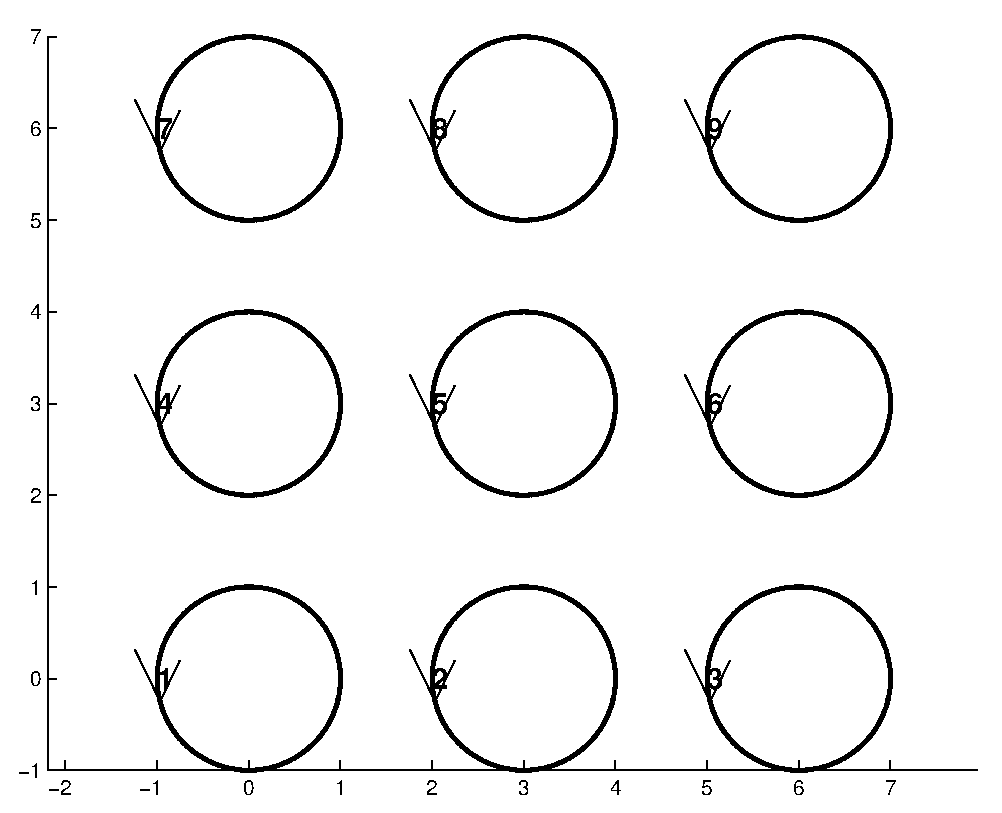
\includegraphics[width=6cm]{circarray}
\caption{An array of $9$ scatterers.}
\label{fig:circarray}
\end{figure}

Let $\Omega$ be the union of disks $D_j$ with radius $r$ whose
midpoints have the coordinates $(an_1^{(j)},an_2^{(j)})\in\mathbb{R}^2$, where
$n_1^{(j)},n_2^{(j)}\in\mathbb{N}$ and $a>0$ is the distance between
two neighboring midpoints. An example for $9$ scatterers is shown in Figure
\ref{fig:circarray}. The PDE is the following.
 
\begin{eqnarray}
\Delta u+k^2u & = & 0  \quad \text{in
}\mathbb{R}^2\backslash\Omega\label{eq:helm0}\\
u&=&0 \quad \text{on } \pO \label{eq:soundsoft0}\\
\frac{\partial u_s}{\partial r}-iku_s & = & o(r^{-1/2}),\label{eq:sommerfeld0}
\end{eqnarray}
Here, $u=u_{inc}+u_s$ is the total field, $u_{inc}$ is the incident
wave, $u_s$ is the scattered field, and $r$ is the radial coordinate.
The Sommerfeld radiation condition
\eqref{eq:sommerfeld} is to be understood to hold uniformly in all
directions. 


We solve the problem using fundamental solutions approximations in
each disk, where the charge  points lie on circles with radius $r_{mfs}<r$.

\subsubsection{Implementation in \mpspack}

\paragraph{Initialization of the problem parameters}

We have the following problem parameters.
\begin{verbatim}
N1=3; N2=3; % Number of scatterers in each direction
r=1; % Radii of circles
a=3; % Distance of midpoints of neighboring circles in each dimension
k=10; % Wavenumber
M=300; % Number of points on each circle
N=150;  % Number of MFS basis fct. in each circle
Rmfs=0.8*r; % Radius of fundamental solutions inside circles
\end{verbatim}

\paragraph{Setup of the geometry}

The geometry is setup using a simple for loop.
\begin{verbatim}
y0=0;
s=segment.empty(N1*N2,0);
for i=1:N1,
    x0=0;
    for j=1:N2
        seg=segment(M,[x0+1i*y0 r 0 2*pi],'p');
        seg.setbc(1,'D',[]);
        s((i-1)*N2+j)=seg;
        x0=x0+a;
    end
    y0=y0+a;
end
\end{verbatim}
In the inner for loop circular segments are created whose handle is
the variable {\texttt seg}. We directly assign the homogeneous
Dirichlet boundary conditions using the command \co{seg.setbc(1,'D',[]);}
The segments are then stored in the array
{\texttt s}. Storing the circular segments in an array makes plotting
easy. Figure \ref{fig:circarray} is simply created with the commands
\begin{verbatim}
o.normals=0;
plot(s,1,o);
\end{verbatim}
Once all segments are created we define the domain by
\co{d=domain([],[],num2cell(s),num2cell(-1*ones(N1*N2,1)));}
This command might look complicated at first because of the use of
{\texttt num2cell}. We need to convert the array {\texttt s} into a
cell structure so that the {\texttt domain} constructor recognizes
that each element of $s$ is a closed shape in itself. Otherwise, the
constructor would try to combine the elements of {\texttt s} into one
connected shape, which is not possible.


\paragraph{Basis functions}

We want to use a basis of fundamental solutions in each of the
circular scatterers. This is achieved with the following for loop.
\begin{verbatim}
x0=0; y0=0; opts.fast=1;
for i=1:N1,
    x0=0;
    for j=1:N2
        Z=@(w) rmfs*exp(2i*pi*w)+x0+1i*y0;
        Zp=@(w) rmfs*2i*pi*w.*exp(2i*pi*w);
        d.addmfsbasis({Z,Zp},N,opts);
        x0=x0+a;
    end
    y0=y0+a;
end
\end{verbatim}
The function handle {\texttt Z} defines the fundamental solutions
curve and {\texttt Zp} its derivative. We have to shift the curves
according to the midpoints of the circles.

\paragraph{Solving the problem}
We now have everything together to setup a problem instance.
This is easily done with the {\texttt
  scattering} class and the following three commands.

\begin{verbatim}
pr=scattering(d,[]);
pr.setoverallwavenumber(k);
pr.setincidentwave(-pi/3);
\end{verbatim}

The solution and timing results are then obtained by
\begin{verbatim}
tic; pr.solvecoeffs; fprintf('\tcoeffs done in %.2g sec\n', toc)
fprintf('\tL2 bdry error norm = %g, coeff norm = %g\n', ...
        pr.bcresidualnorm, norm(pr.co));
\end{verbatim}
On a standard Core 2 Duo Laptop this takes just under $40$
seconds with a boundary error of about $2\cdot 10^{-13}$.
We can plot the solution using the following commands.
\begin{verbatim}
o.bb=[-a N2*a -a N1*a];
o.dx=0.05;
o.sepfigs=1;
pr.showthreefields(o);
\end{verbatim}
The command {\texttt pr.showthreefields(o)} plots the incoming wave,
scattered field and full field using the parameters given in {\texttt
  o}. We have specified {\texttt o.sepfigs=1}. This creates three
separate figures for the three different fields instead of plotting
everyhting into one figure.

\begin{figure}
\center
\begin{tabular}{cc}
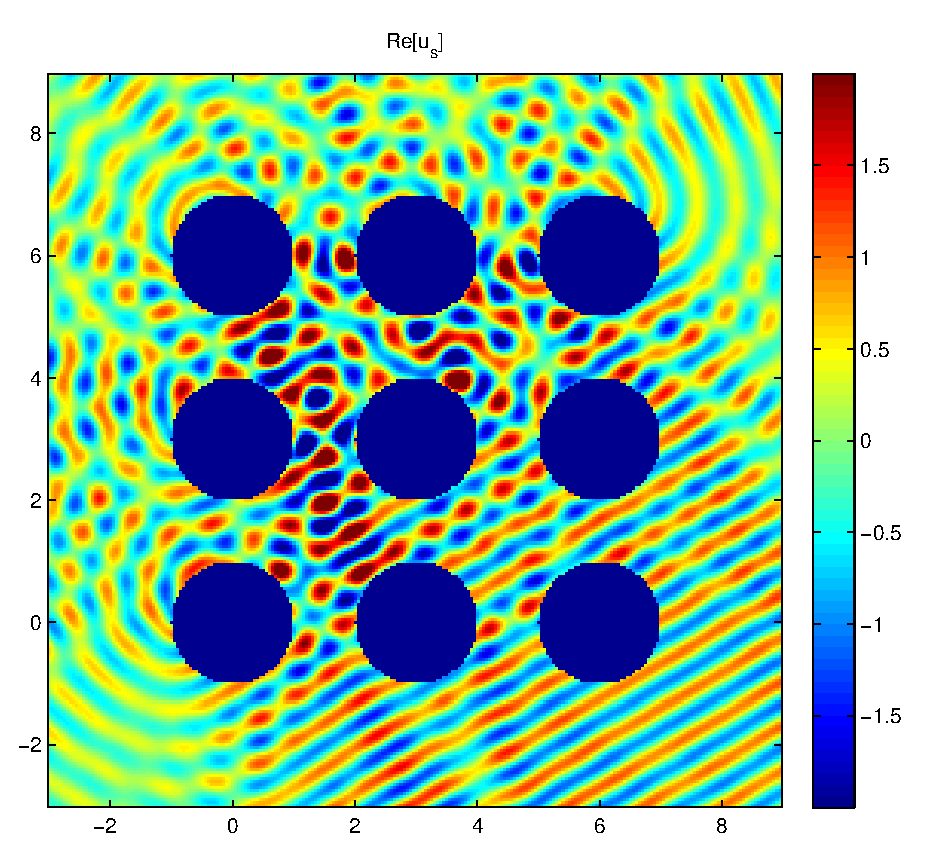
\includegraphics[width=6cm]{circarrayscattered} &
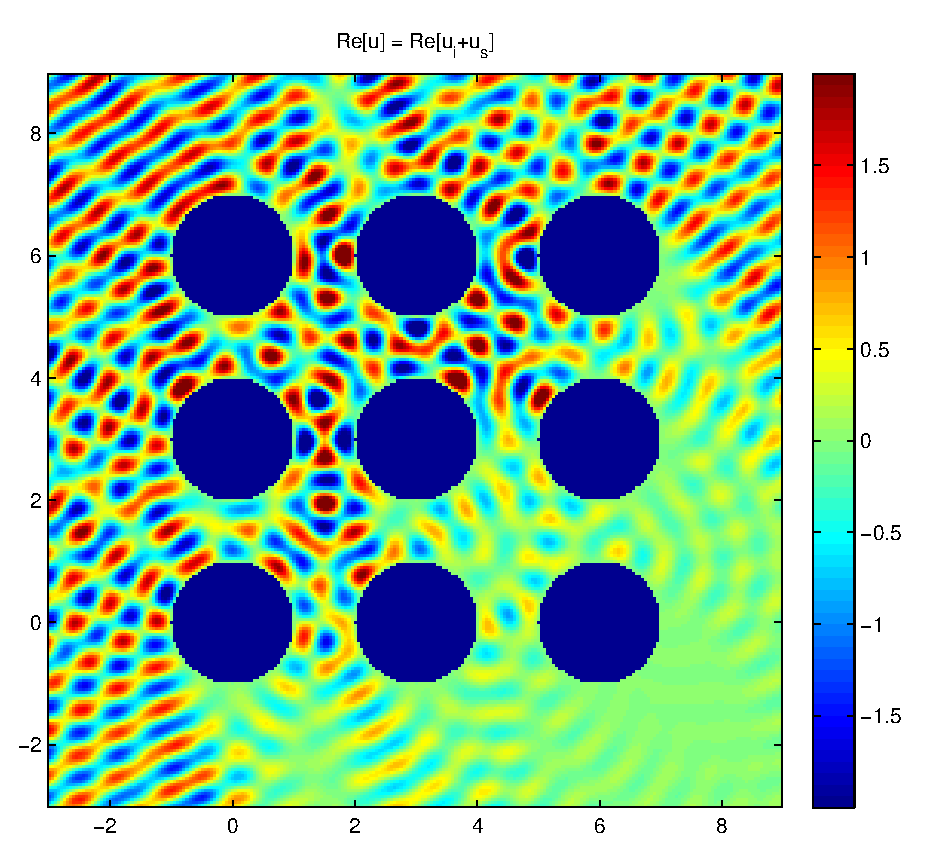
\includegraphics[width=6cm]{circarrayfull}
\end{tabular}
\caption{The scattered (left) and the full field (right) for the
  problem of scattering from an array of circles.}
\label{fig:circarraysol}
\end{figure}


The scattered and the full field are shown in Figure
\ref{fig:circarraysol}. Note that plotting can take a long time since
the array of scatterers spans many wavelenghts for which we need a
sufficiently high resolution. The solution is not symmetric with
respect to the diagonal since the incident angle for the incoming wave is
$-\frac{\pi}{3}$, destroying the symmetry given by the configuration
of scatterers.














\bfi % ffffffffffffffffffffffffffffffffffffffffffffffffffffffffffffffffffffff
\ig{width=\textwidth}{dielhole.eps}
\ca{Transmission scattering (TE-polarized) from dielectric with two inclusions: an air hole
(to the right side) and a `metallic' PMC inclusion (to the left side).
Multiple MFS basis curves are used.
Left: incident wave $u_{inc}$. Center: scattered wave
$u_s$. Right: their sum, the total solution field $u$.}{f:dielhole}
\efi
\bfi % ffffffffffffffffffffffffffffffffffffffffffffffffffffffffffffffffffffff
\bc\ig{width=0.6\textwidth}{dielholegeom.eps}\ec
\ca{MFS curves (red) and boundary curves (blue) used for transmission scattering from dielectric with two inclusions.}{f:dielholegeom}
\efi

% ===========================================================================
\subsection{Transmission scattering with `metal' and air holes}
\label{s:dielhole}

Here we demonstrate how the fundamental solutions introduced in
Sec.~\ref{s:ext} can be used to solve efficiently
the scattering of TE (transverse-electric) polarized $z$-invariant
plane-wave (2D Maxwell equations) from a smooth dielectric body with various
inclusions. We will be somewhat brief in this example.

The mathematical set up is identical to the previous example, except that
there is a bounded dielectric region which has refractive index $n = 1.5$ and
hence a Helmholtz solution with
larger wavenumber than in the surrounding vacuum (or `air').
The field $u$ represents $H_z$, the out-of-plane magnetic field.
The solution in the dielectric must match that in the air at their common
boundary, as we describe shortly. We also have a homogeneous boundary condition
on a `metallic' inclusion inside the dielectric; see Fig.~\ref{f:dielhole}.

First we set up some curves, formed by scaling, translating and rotating
standard `radius-1' segments {\tt 's'} and {\tt 'c'}, and build the
three domains from them,
\begin{verbatim}
s = segment.smoothstar(200, 0.2, 3);          % weak trefoil shape
c = segment.smoothstar(70, 0.1, 2);           % squashed circle

sd = s.scale(2);                              % outer bdry of dielectric
sa = translate(rotate(sm,.3), .8);            % air inclusion bdry
sm = c.scale(0.5); sm.rotate(pi/5); sm.translate(-.8-.6i); % 'metal' bdry

de = domain([], [], sd, -1);                  % exterior air domain
da = domain(sa, 1);                           % air inclusion domain
d = domain(sd, 1, {sm sa}, {-1 -1});          % dielectric w/ 2 holes
d.setrefractiveindex(1.5);                    % choose dielectric index
\end{verbatim}

Assuming relative permeability of unity, the relative
permittivity of the dielectric is $\epsilon = n^2$.
The transverse-electric (TE) boundary condition is that $u$ is continuous
across a dielectric interface (segments {\tt sd} and {\tt sa}),
while for the normal derivative $\epsilon^{-1} \partial u/\partial \nu$ is
continuous.\footnote{See \cite{jackson}.
See {\tt segment.dielectriccoeffs} for where this
is set up in \mpspack.}
We set this up, and a Dirichlet BC on the other inclusion, with,
\begin{verbatim}
setmatch([sd sa], 'diel', 'TE');        % impose TE matching diel-air
sm.setbc(1, 'D', []);                   % Dirichlet (PMC) BC on 'metal'
\end{verbatim}

The domains are then collected into a scattering problem as follows (note
that by including {\tt da} in the first argument list, it is set up as an
`air' domain thus receives a nonzero $u_{inc}$ plane-wave field, although
results are similar if {\tt de} is the only air domain),
\begin{verbatim}
pr = scattering([de da], d);   % includes air pocket in nonzero u_inc
pr.setoverallwavenumber(8);    % incident (air) wavenumber
pr.setincidentwave(-pi/3);     % if just angle given, assumed plane wave
\end{verbatim}

MFS bases are very convenient for such analytic boundaries, and we use the
analytic continuation of the boundary parametrization to generate MFS curves
either inside or outside the actual segment curves
({\tt tau>0} is inside, and {\tt tau<0} outside, for CCW segments).
Fig.~\ref{f:dielholegeom} shows the five MFS curves and the three segments.
The reason the dielectric needs three MFS curves is that (analogous
with Runge's Theorem in complex approximation), singularities are needed in
{\em each} disconnected component of the domain's complement.
The distances {\tt tau} in the following should be chosen as large as possible
while still keeping the coefficient norm {\tt norm(pr.co)} not too large
(i.e.\ $10^4$ or less).
\begin{verbatim}
de.addmfsbasis(sd, 120, struct('tau',0.05)); % BASIS SETS: exterior domain
da.addmfsbasis(sa, 60, struct('tau',-0.1)); % inside air pocket
d.addmfsbasis(sd, 150, struct('tau',-0.05)); % 1st of 3 curves for diel...
d.addmfsbasis(sm, 60, struct('tau',0.1));   % ...2nd curve in `metal' hole
d.addmfsbasis(sa, 60, struct('tau',0.1));   % ...3rd curve in air hole
\end{verbatim}
Note that the basis set degrees were optimized roughly for this $k$ value,
giving only 450 total degrees of freedom for a problem around
8 wavelengths in size.
Solving for the coefficients of the solution takes 0.67 sec,
\begin{verbatim}
pr.solvecoeffs; pr.bcresidualnorm
\end{verbatim}
The $L^2$ boundary error is less than $10^{-7}$.
We then plot the incident, scattered, and total field as usual with
{\tt pr.showthreefields;} giving Fig.~\ref{f:dielhole}.
Computing the solution on a 400$\times$400 grid takes 11 sec.

\subsubsection{Convergence study}
Once a good set of MFS basis sizes has been chosen, as above, they
may all be changed at once conveniently with the {\tt nmultiplier} option.
We redo the basis sets as follows,
\begin{verbatim}
d.clearbases; de.clearbases; da.clearbases;
de.addmfsbasis(sd, [], struct('tau',0.05,'nmultiplier', 120/450));
da.addmfsbasis(sa, [], struct('tau',-0.1,'nmultiplier', 60/450));
d.addmfsbasis(sd, [], struct('tau',-0.05, 'nmultiplier', 150/450));
d.addmfsbasis(sm, [], struct('tau',0.1, 'nmultiplier', 60/450));
d.addmfsbasis(sa, [], struct('tau',0.1, 'nmultiplier', 60/450));
\end{verbatim}
The mutipliers were set up to be the fraction of the total degrees of freedom
that they were above, but now they can be scaled with a single command,
viz, {\tt pr.updateN(450)} sets up the original basis sizes,
as may be checked with {\tt diff([pr.basnoff pr.N])} which gives the
numbers of degrees of freedom in each problem basis set.
We put this in a convergence loop,
\begin{verbatim}
Ns=300:50:600; for i=1:numel(Ns)
  pr.updateN(Ns(i)); pr.solvecoeffs;
  fprintf('N=%d, co-norm=%g, bc-norm=%g, u(0)=%.16g\n', Ns(i), ...
      norm(pr.co), pr.bcresidualnorm, pr.pointsolution(pointset(0)));
end
\end{verbatim}
Note that we doubled the number of quadrature points on the original
domains to perform this high-accuracy study, giving 680 quadrature points in
total.
The output is as follows,
\begin{verbatim}
N=300, co-norm=2125.38, bc-norm=0.000363003, |u(0)|=3.045222448551815
N=350, co-norm=1968.37, bc-norm=1.26165e-05, |u(0)|=3.045222451567895
N=400, co-norm=1844.05, bc-norm=4.21908e-07, |u(0)|=3.045222451435764
N=450, co-norm=1746.25, bc-norm=9.77848e-08, |u(0)|=3.045222451435782
N=500, co-norm=1651.79, bc-norm=3.96167e-09, |u(0)|=3.045222451436035
N=550, co-norm=1581.87, bc-norm=1.1487e-09,  |u(0)|=3.045222451436006
N=600, co-norm=1521.16, bc-norm=1.44025e-10, |u(0)|=3.045222451436037
\end{verbatim}
This suggests convincingly
that, at least for $u$ at the origin, we had 12 correct
digits in the solution with the total $N=450$ used above,
and probably achieved 14 digits with $N=600$,
computed in just a few seconds.




% ===========================================================================
\subsection{Acoustic scattering from the unit square}
\label{s:square}

This example introduces a new feature: the use of decomposition
of a region of constant wavenumber into computational subdomains connected
by fictitious boundaries. The code is in \verb?examples/tut_square.m?

\subsubsection{Problem description and solution approach}
\label{s:scatbvp}

In this example we solve the problem of time-harmonic 
acoustic sound-soft scattering from the unit square $\Omega=(-0.5,0.5)^2$.
The full PDE has the following form.
\begin{eqnarray}
\Delta u+k^2u & = & 0  \quad \text{in
}\mathbb{R}^2\backslash\Omega\label{eq:helm}\\
u&=&0 \quad \text{on } \pO \label{eq:soundsoft}\\
\frac{\partial u_s}{\partial r}-iku_s & = & o(r^{-1/2}),\label{eq:sommerfeld}
\end{eqnarray}
Here, $u=u_{inc}+u_s$ is the total field, $u_{inc}$ is the incident
wave, $u_s$ is the scattered field, and $r$ is the radial coordinate.
The Sommerfeld radiation condition
\eqref{eq:sommerfeld} is to be understood to hold uniformly in all
directions. 

\begin{figure}
\center
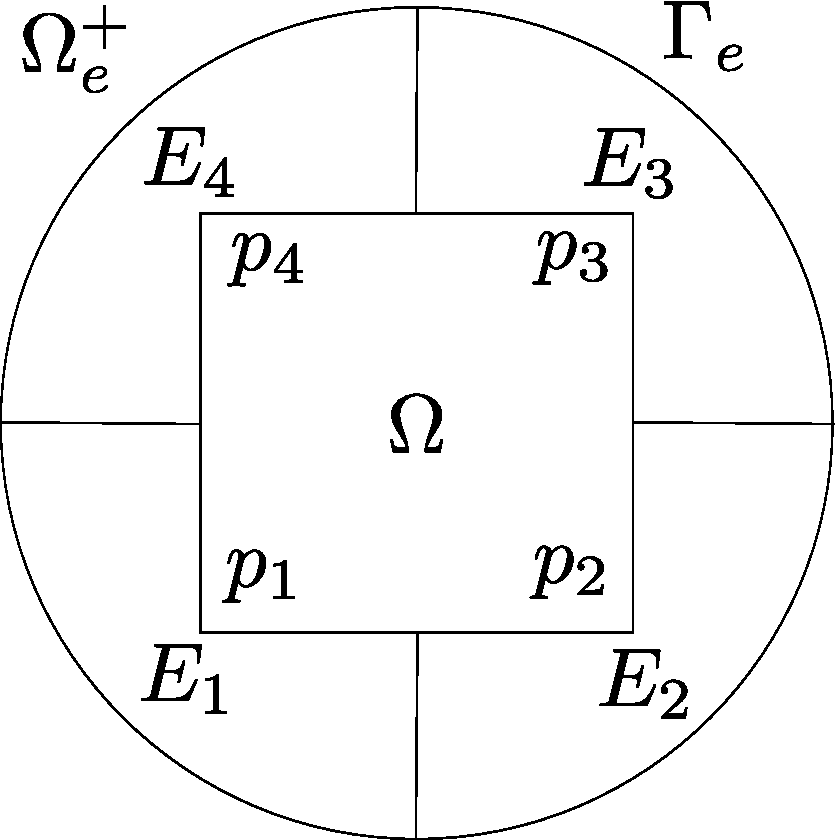
\includegraphics[width=6cm]{geometry}
\vspace{-.5cm}
\caption{Geometry of the problem}
\label{fig:geom}
\end{figure}


To achieve high accuracy we cannot simply use fundamental solutions
to approximate the scattered field. The problem is the singularities
of the solution $u$ at the corners. If these are not represented in
the basis our approximation error will decay very slowly as the number
of basis functions increases. To solve this problem we use the domain
decompositon shown in Figure \ref{fig:geom}. The idea is that each of
the elements $E_i$ only contains one corner $p_i$ of the square. We can then
match the corner behavior in each domain by using fractional order
Bessel functions. Since furthermore, $u=0$ on $\partial\Omega$ it will
be sufficient to use Fourier-Bessel sine functions that automatically
satisfy the zero boundary conditions on the sides of the square.
Hence, the total field $u$ is approximated in each element $E_i$ using
an approximation of the form
$$
u(r,\theta)\approx
\sum_{j=1}^{N_i}c_j^{(i)}J_{\frac{2}{3}j}(kr)\sin(\frac{2j}{3}\theta).
$$
The polar coordinate system in each element $E_i$ is rotated in such a way
that the basis functions are zero on the sides adjacent to the corner
at $p_i$.

In the infinite domain $\Omega_e^+$ we use a basis of fundamental
solutions to represent the scattered field $u_s$. Hence, for
$\bx\in\Omega^+$ we have
$$
u_s(\bx)\approx \sum_{j=1}^{N_e}\frac{i}{4}c_j^{(e)}H_0^{(1)}(|\bx-\by_j|),
$$
where $\by_j=r_{mfs}e^{i\phi_j}$ and $\phi_j=\frac{2\pi j}{N_e}$. Note
that we approximate with the fundamental solutions the scattered field
$u_s$ while in the finite subdomains $E_i$ we approximate the total
field $u$. The compatibility conditions between approximations $u^{i}$
und $u^{j}$ in two neighboring elements $E_i$ and $E_j$ with common
boundary $\Gamma_{ij}$ are given by
$$
u^{(i)}(\bx)\approx u^{(j)}(\bx),\quad \frac{\partial u}{\partial
  n_i}{u^{(i)}}(\bx)\approx  \frac{\partial u}{\partial
  n_i}{u^{(j)}}(\bx),
$$
where $\bx\in\Gamma_{ij}$ and $\frac{\partial}{\partial\nu_i}$ is the
outward normal derivative at the boundary of $E_i$.
On the interface $\Gamma_{ie}$ between an element $E_i$ and the
exterior domain $\Omega_e^{+}$ we have the compatibility conditions
$$
u^{(i)}(\bx)\approx u_{inc}(\bx)+u_s^{(e)}(\bx),\quad \frac{\partial}{\partial
  n_i}{u^{(i)}}(\bx)\approx  \frac{\partial}{\partial
  n_i}{(u_s^{(e)}+u_{inc})}(\bx),
$$
where $u_s^{(i)}$ is the fundamental solutions approximation to the
scattered field in $\Omega_e^{+}$. We have to add the incident field
to the approximate scattered field since we are matching with the
total field in the elements $E_i$.
An approximate solution to the whole problem is now 
computed by minimizing the $L^2$ error of 
the compatibility conditions on all interfaces.

\subsubsection{Implementation in \mpspack}

Although the setup of the problem seems quite complicated we will see
that it is very simple to set it up in \mpspack. Indeed, the most part
of the code will be devoted to creating the mesh structure from
Figure \ref{fig:geom}.

\paragraph{Initialization of the problem parameters}

We need to define the following problem parameters.
\begin{verbatim}
k = 50;      % Wavenumber
r = 1.0;     % Radius of outer circle    
M = 200;     % Number of quadrature points on segments
N=100;       % Number of basis fct. in each subdomain
a=.5;        % Half-Size of the square
rmfs=0.8*r;  % Radius of the fundamental solutions curve
\end{verbatim}


\paragraph{Setup of the geometry}

We now need to define the geometry. Fortunately,
\mpspack\ gives some support for the construction of the geometry.

The list of segments is defined by the following three commands.

\begin{verbatim}
s = segment.polyseglist(M, [1i*r 1i*a a+1i*a a r]);
s=[s(1:3) segment(2*M, [0 r 0 pi/2])];
s = [s rotate(s, pi/2) rotate(s, pi) rotate(s, 3*pi/2)];
\end{verbatim}
The first command defines all the straight lines that form part of the
boundary of $E_3$. For this we use {\texttt{polyseglist}}. The command
{\texttt polyseglist} constructs a closed polygon. We then delete the
last two segments of the array {\texttt s} and add instead the
circular line segment. This results in the segments shown in the left
plot of Figure \ref{fig:circelem}. We now rotate this element three times to
obtain the segments showin in the right plot of Figure \ref{fig:circelem}.
\begin{figure}
\begin{tabular}{cc}
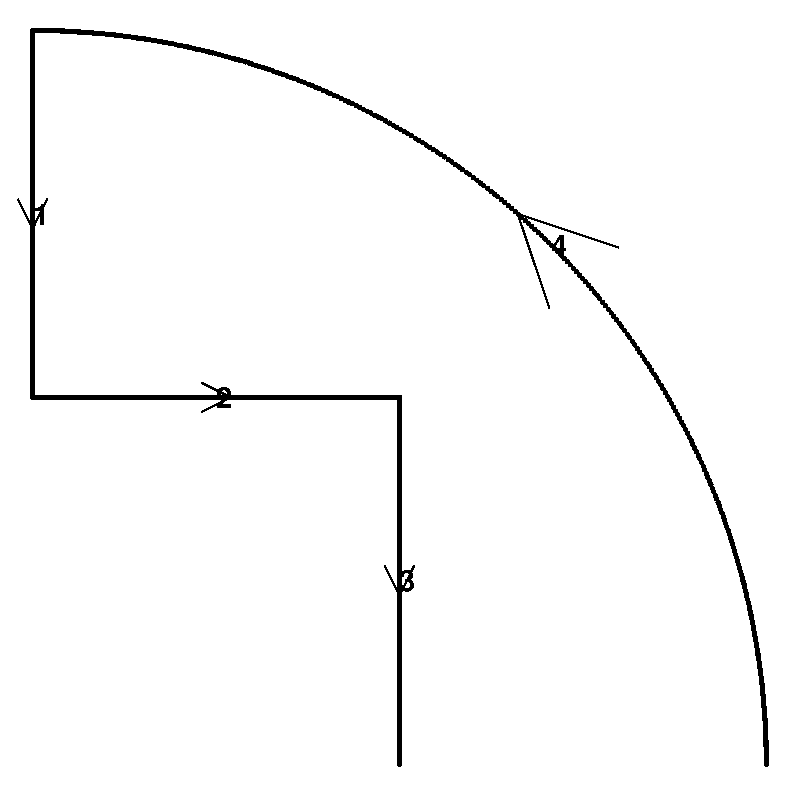
\includegraphics[width=5cm]{circelem1} &
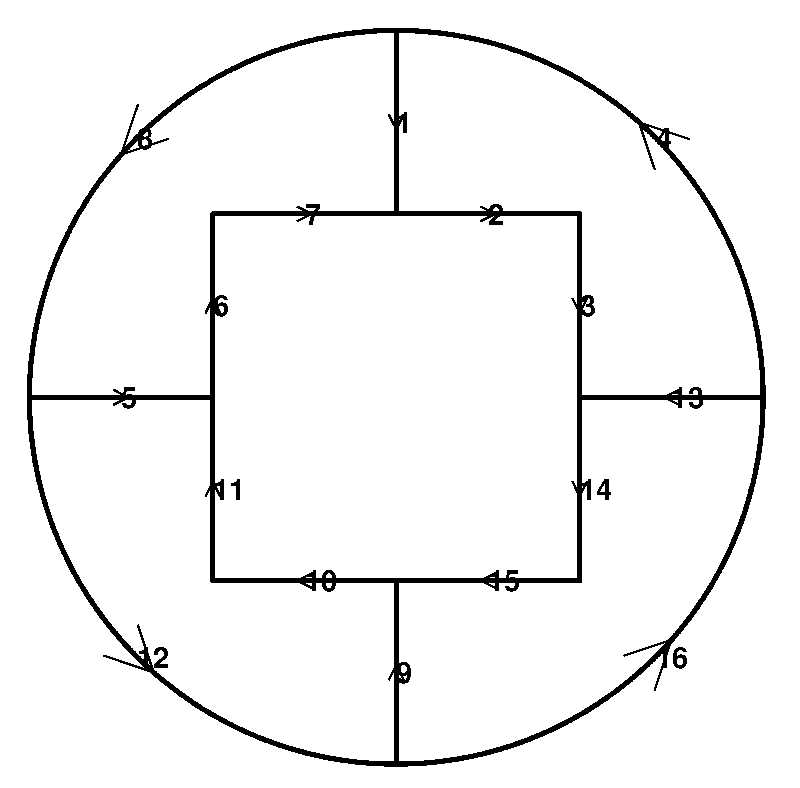
\includegraphics[width=5cm]{circelem2}
\end{tabular}
\caption{The segments in the right plot are created by rotating the segments
  shown in the left plot.}
\label{fig:circelem}
\end{figure}

For later it is important to have a separate list of all segments not
belonging to the square and all segments belonging to the outer
circle.

\begin{verbatim}
sdecomp=s([1 4 5 8 9 12 13 16]); % All artificial boundaries
extlist=s([4 8 12 16]);          % Segments forming the outer circle
\end{verbatim}

We now define the domains. By taking the rotational symmetry into
account we can do this in a simple for loop.

\begin{verbatim}
d=domain.empty(4,0);
for j=1:4, d(j)=domain(s(1+mod(4*(j-1)+[0 1 2 12 3],16)),[1 1 1 -1 1]); end
ext = domain([], [],extlist(end:-1:1), -1); 
\end{verbatim}
The for loop looks slightly complicated. But all it does is pick out
the right indices for the elements forming a domain and creating it
together with the right sense of direction. At the end we have an
array {\texttt d} containing the four fine domains $E_i$. The exterior
domain {\texttt ext} is created by traversing {\texttt extlist} in
reverse order with reversed sense $-1$. This is necessary since we now
have the boundary of an exterior domain, which has a reversed sense of
direction.

\paragraph{Boundary conditions and basis functions}

Setting up the compatibility conditions between the elements is 
trivial. It is done by
the command
\begin{verbatim}
sdecomp.setmatch([k -k],[1 -1]);
\end{verbatim}
The matching conditions for the function values are scaled by the
wavenumber $k$ to balance the different scaling between the $L^2$ error
in the function and the $L^2$ error in the
derivative.\footnote{Consider the one dimensional plane wave
  $e^{ikx}$. The derivative is $ike^{ikx}$. Hence, in general it makes sense to
  scale the $L^2$ error of function values by $k$ to give it the same
  dimension as the $L^2$ error of the derivative.}

We can now add the basis functions to the domains. The fractional
Bessel functions are added to the interior domains by the following
command.
\begin{verbatim}
nuopts=struct('type','s','cornermultipliers',[0 0 1 0 0],'rescale_rad',1);
for j=1:4, d(j).addcornerbases(N,nuopts); end
\end{verbatim}
The options structure {\texttt nuoopts} specifies that we only want
Fourier-Bessel sine functions at the third corner of each domain. This
is the corner belonging to the square. The option {\texttt
  'rescale\_rad'} specifies that the basis functions are rescaled to
balance out the bad scaling of Bessel functions. The method {\texttt
  addcornerbases} automatically finds out the right fractional orders,
offsets and suitable branch vectors.

The exterior fundamental solutions are added with the following command.
\begin{verbatim}
Z=@(t) rmfs*exp(2i*pi*t); Zp=@(t) 2i*pi*rmfs*exp(2i*pi*t);
opts=struct('eta','k','fast',1,'nmultiplier',2);
ext.addmfsbasis({Z, Zp},N,opts);
\end{verbatim}
Note that now {\texttt nmultiplier} is set to $2$. It turns out to be
effective for this problem to use twice as many fundamental solutions
as there are Fourier-Bessel sine functions in each domain.

\paragraph{Solving the problem}
We now have everything together to setup the problem class and solve
the scattering problem. The following commands setup the scattering
problem and define an incident plane wave.
\begin{verbatim}
pr=scattering(ext,d);
pr.setoverallwavenumber(k);
pr.setincidentwave(-pi/4);
\end{verbatim}
There is one small specialty here. In the first line we have 
defined {\texttt ext} to be an air-domain and the array {\texttt d} to
be a non-air domain. This tells \mpspack\ to add the incident field to
the exterior basis functions in assembling the least-squares
problem. In the finite domains this is not necessary since there we
approximate directly the full field.



The following commands now solve the problem and plot the solution
$u$.
\begin{verbatim}
tic; pr.solvecoeffs; fprintf('\tcoeffs done in %.2g sec\n', toc)
fprintf('\tL2 bdry error norm = %g, coeff norm = %g\n', ...
        pr.bcresidualnorm, norm(pr.co))
o.bb=[-1.5 1.5 -1.5 1.5];
o.dx=0.02;

[ui gx gy] = pr.gridincidentwave(o);
u = pr.gridsolution(o);

figure;
imagesc(gx, gy, real(ui+u)); title('Full Field (Real Part)');
c = caxis; caxis([-1 1]*max(c));
axis equal tight;
colorbar;
set(gca,'ydir','normal'); 
\end{verbatim}
The incident field {\texttt ui} 
is automatically evaluated only in air-domains. If
we want to evaluate it in all domains we have to set {\texttt
  o.all=1}. But here the default behavior is fine for us. The sum
{\texttt ui+u} is now the total field in all domains (remember that
{\texttt u} approximates the total field in the interior domains
and the scattered field in the exterior domain). The {\texttt
  scattering} class also provides a routine {\texttt showthreefields}
to plot the incident wave, scattered field and total field. However,
the routine assumes that the computed solution is the scattered field,
which is not correct for the way we have set up this problem. The
resolution if the plot can easily be increased by decreasing the
variable {\texttt o.dx}, which influences the distance of two grid points.


The output of the example problem is shown in Figure \ref{fig:squareplot}.
\begin{figure}
\center
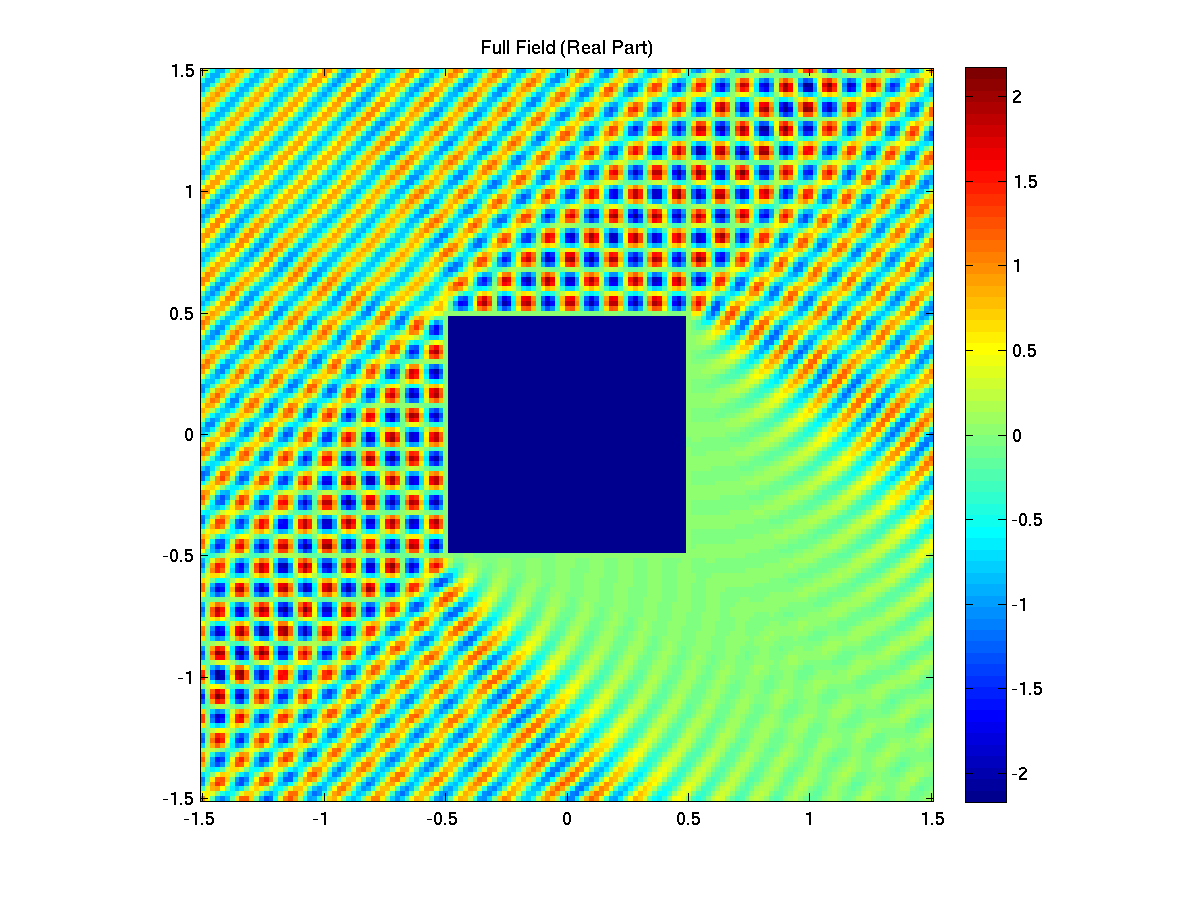
\includegraphics[width=8cm]{squareplot}
\caption{The solution of the scattering problem on the unit
  square with sound-soft boundary conditions.}
\label{fig:squareplot}
\end{figure}
The $L^2$ boundary error of the solution is approximately $1.5\cdot
10^{-10}$. On a standard laptop with Intel Core 2 Duo processor the
solution vector is computed in around $11$ seconds. The plot takes
slightly longer.

A wonderful feature of this approach is that we can trivially switch
to a sound-hard scattering problem, that is instead of requiring $u=0$
on $\partial\Omega$ we require $\frac{\partial}{\partial n} u=0$ on
$\partial\Omega$. All we have to do is switch to Fourier-Bessel cosine
functions. These automatically satisfy the required condition for the
normal derivative. The solution to this problem is shown in Figure
\ref{fig:squareplot2}.
\begin{figure}
\center
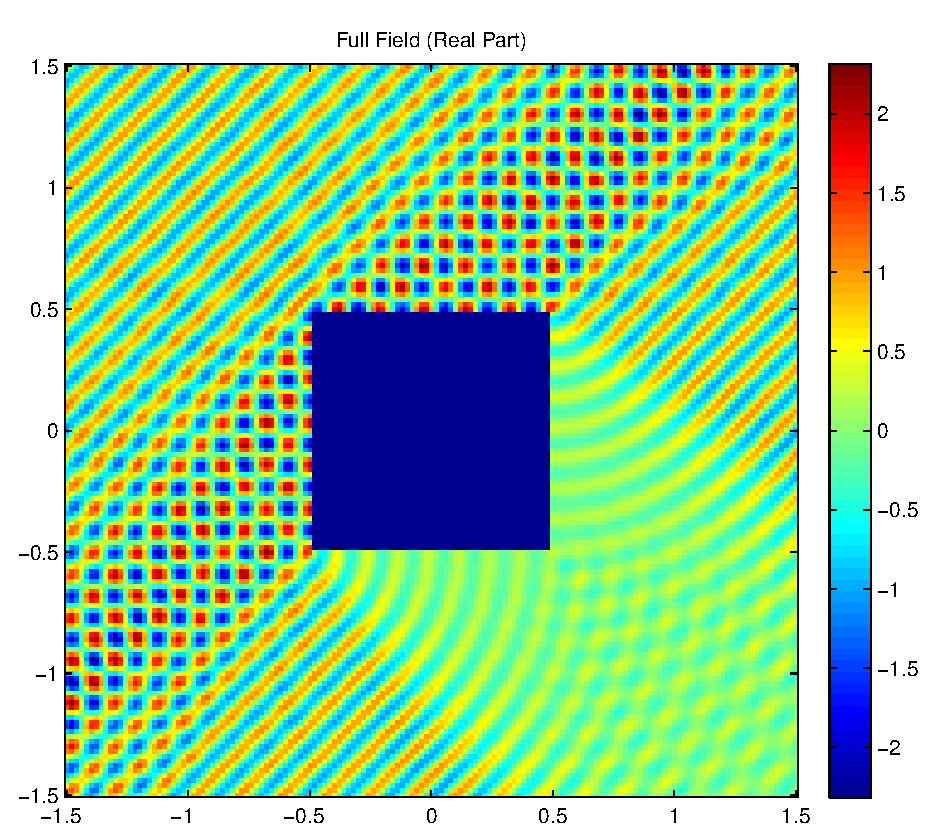
\includegraphics[width=8cm]{squareplot2}
\caption{The solution of the scattering problem on the unit
  square with sound-hard boundary conditions.}
\label{fig:squareplot2}
\end{figure}
The accuracy and solution time are comparable to the sound-soft
scattering case.

%%% Local Variables: 
%%% mode: latex
%%% TeX-master: "tutorial"
%%% End: 



\bibliographystyle{siam} 
\bibliography{alexrefs}
\end{document}
